\section{Observation and Calculations}

\subsection{Op-amp as an integrator}
    
Refer Fig. \ref{intexp}.

    \begin{itemize}
        \item $R_1 = 9.85$ \kohm, $R_2 = 9.90$ \kohm, $R_f = 99.10$ \kohm
        \item $C_f = 102.2$ nF\\
    \end{itemize}

    The following waveforms were obtained on the oscilloscope.

    \begin{figure}[H]
        \centering
        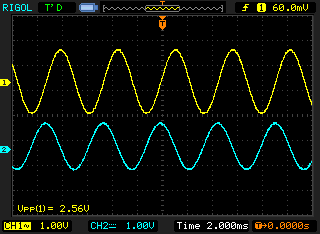
\includegraphics[width=0.75\columnwidth]{images/int5.png}
        \caption{Sinusoidal input waveform (above) and its corresponding phase shifted output waveform (below) by an Integrator Circuit}
        \label{int1}
    \end{figure}

    \begin{figure}[H]
        \centering
        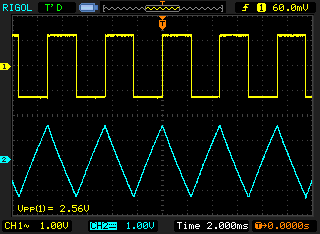
\includegraphics[width=0.75\columnwidth]{images/int2.png}
        \caption{Square wave input signal (above) and its corresponding output waveform (below) by an Integrator Circuit.}
        \label{int2}
    \end{figure}

    In Fig. \ref{int2}, the input may be treated as $\pm V$ for short periods of time. With time, the area swept out from underneath the input signal increases, and then decreases due to the polarity changes. It follows that the output will grow (or shrink) in a linear fashion, as the input is constant. In other words, straight ramps are produced, hence this type of circuit is also known as the \textit{Ramp Generator}.

    \begin{figure}[H]
        \centering
        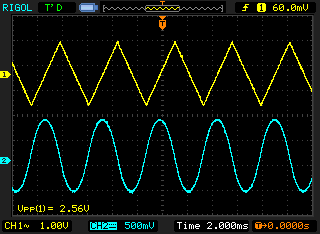
\includegraphics[width=0.75\columnwidth]{images/int3.png}
        \caption{Triangle waveform input (above) and its corresponding output waveform (below) by an Integrator Circuit}
        \label{int3}
    \end{figure}

    In Fig. \ref{int3}, the triangular wave is composed of linearly raising and linearly falling parts, the integral of which will result in a quadratic term along with some constants arising due to the components of the circuit. So the output will be parabolic in nature. The output observed is a composition of +ve and -ve halves of \textit{parabolas}, and \textit{not a sinusoidal curve}.

% ======================================================================================

\subsection{Op-amp as a differentiator}
    Refer Fig. \ref{diffexp}.
    \begin{itemize}
        \item $R_1 = 1.006$ \kohm, $R_2 = 1.002$ \kohm, $R_f = 9.90$ \kohm
        \item $C_f = 10.40$ nF, $C_\text{in} = 102.2$ nF\\
    \end{itemize}
    The following waveforms were obtained on the oscilloscope.

    \begin{figure}[H]
        \centering
        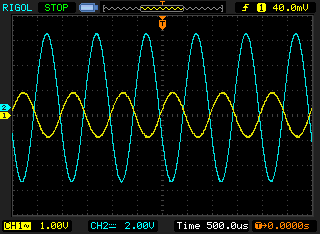
\includegraphics[width=0.75\columnwidth]{images/diff01.png}
        \caption{Sinusoidal input waveform with its corresponding output waveform (shown here with lower amplitude), phase shifted by $\pi$, by a differentiator circuit}
        \label{diff1}
    \end{figure}

    \begin{figure}[H]
        \centering
        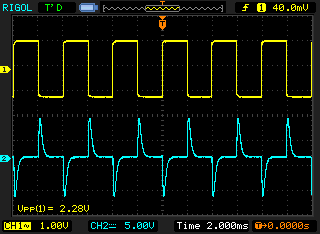
\includegraphics[width=0.75\columnwidth]{images/diff3.png}
        \caption{Square wave input signal (above) with its corresponding output signal. The positive and negative spikes coincide with the rising/falling edge of the input square wave, which indicate increasing/decreasing slope.}
        \label{diff2}
    \end{figure}

    \begin{figure}[H]
        \centering
        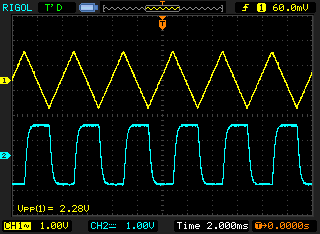
\includegraphics[width=0.75\columnwidth]{images/diff23.png}
        \caption{Triangular wave input signal (above) with its corresponding output signal. Since the input consists of steady increase/decrease in voltage, the corresponding slopes are constant, resulting in a square wave.}
        \label{diff3}
    \end{figure}

    \begin{figure}[H]
        \centering
        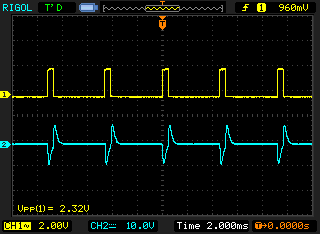
\includegraphics[width=0.75\columnwidth]{images/diff4.png}
        \caption{Pulsating input signal (above) with the corresponding output signal by a differentiator circuit. The same explanation as Fig. \ref{diff2} applies here.}
        \label{diff4}
    \end{figure}

% ======================================================================================
\subsection{Op-amp as an active low pass filter}
    Using the circuit in Fig \ref{lowpasscircuit}, the following values voltages were obtained as a function of frequency.

    \begin{itemize}
        \item $R_1 = 9.85$ \kohm, $R_f = 99.10$ \kohm, $C = 102.2$ nF
        \item $f_c=1/2 \pi RC=158$ Hz\\
    \end{itemize}
    
    \begin{table}[H]
    \centering
    \begin{tabular}{|c|c|c|c|} \hline
        Frequency & $V_o$ (V) & $A_v = V_o/V_i$ & Gain (in dB) \\ \hline
        2.5 Hz       & 15.4   & 9.87 &  45.79 \\
        4.0 Hz       & 15.4   & 9.87 &  45.79 \\
        8.7 Hz       & 15.2   & 9.74 &  45.53 \\
        9.9 Hz       & 15.2   & 9.74 &  45.53 \\
        13.55 Hz     & 15.2   & 9.74 &  45.53 \\
        25.0 Hz      & 15.0     & 9.62 &  45.27 \\
        36.0 Hz      & 14.6   & 9.36 &  44.73 \\
        43.5 Hz      & 14.2   & 9.10 &  44.17 \\
        56.0 Hz      & 14.2   & 9.10 &  44.17 \\
        74.0 Hz      & 13.8   & 8.85 &  43.60 \\
        93.0 Hz      & 13.2   & 8.46 &  42.71 \\
        111.5 Hz     & 12.5   & 8.01 &  41.62 \\
        127.0 Hz     & 11.9   & 7.63 &  40.64 \\
        145.0 Hz     & 11.4   & 7.31 &  39.78 \\
        153.0 Hz     & 11.0     & 7.05 &  39.06 \\
        158.0 Hz     & 10.8   & 6.92 &  38.70 \\
        176.0 Hz     & 10.4   & 6.67 &  37.94 \\
        186.0 Hz     & 10.0     & 6.41 &  37.16 \\
        196.0 Hz     &  9.6   & 6.15 &  36.34 \\
        215.0 Hz     &  9.1   & 5.83 &  35.27 \\
        228.0 Hz     &  8.6   & 5.51 &  34.14 \\
        260.0 Hz     &  7.8   & 5.00    &  32.19 \\
        300.0 Hz     &  7.2   & 4.62 &  30.59 \\
        355.0 Hz     &  6.08  & 3.9  &  27.21 \\
        375.0 Hz     &  5.76  & 3.69 &  26.13 \\
        415.0 Hz     &  5.28  & 3.38 &  24.38 \\
        465.0 Hz     &  5.0     & 3.21 &  23.30 \\
        500.0 Hz     &  4.6   & 2.95 &  21.63 \\
        550.0 Hz     &  4.2   & 2.69 &  19.81 \\
        620.0 Hz     &  4.0    & 2.56 &  18.83 \\
        695.0 Hz     &  3.6   & 2.31 &  16.72 \\
        805.0 Hz     &  3.0     & 1.92 &  13.08 \\
        980.0 Hz     &  2.6   & 1.67 &  10.22 \\
        1.325 kHz    &  2.0     & 1.28 &   4.97 \\
        1.62 kHz    &  1.56  & 1.00    &   0.00    \\
        2.00 kHz    &  1.24  & 0.79 &  -4.59 \\
        2.55 kHz    &  1.00     & 0.64 &  -8.89 \\
        5.05 kHz    &  0.52  & 0.33 & -21.97 \\
        8.00 kHz    &  0.36  & 0.23 & -29.33 \\
        14.90 kHz   &  0.18  & 0.12 & -43.19 \\
        30.75 kHz   &  0.108 & 0.07 & -53.41 \\
        80.00 kHz   &  0.072 & 0.05 & -61.52 \\
        307.50 kHz  &  0.060 & 0.04 & -65.16 \\
        515.00 kHz  &  0.050 & 0.03 & -68.81 \\
        1.00 MHz &  0.050  & 0.03 & -68.81 \\
        3.00 MHz &  0.050  & 0.03 & -68.81 \\
        \hline
        \end{tabular}    
        \caption{Frequency response data for op-amp as an active low pass filter}
        \label{tab:1}
\end{table}
    
    \begin{figure}[H]
        \centering
        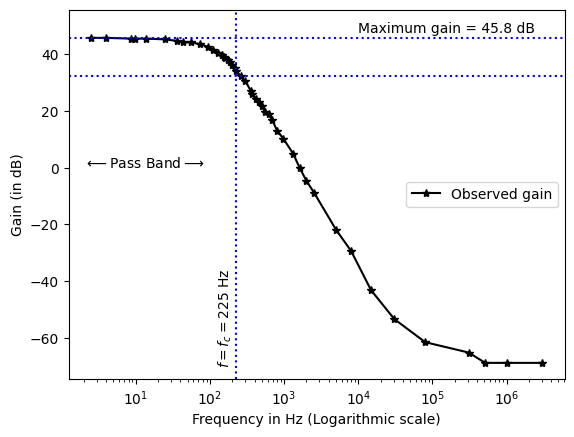
\includegraphics[width=0.81\columnwidth]{images/low_pass_output.png}
        \caption{Bode plot (Gain vs frequency) for Table \ref{tab:1}}
        \label{lowoutput}
    \end{figure}

From the graph, the observed value of the cutoff frequency is 225 Hz. There is some deviation in the expected value from the experimental value, which could be due to various reasons like offset voltage or error in measurement.

% ======================================================================================
\subsection{Op-amp as an active high pass filter}
By constructing a high pass filter (Fig. \ref{highpasscircuit}), the following values voltages were obtained as a function of frequency. Note: $C_f$ was not connected in parallel to $R_f$ in the practical circuit used as it attenuated higher frequencies. 

    \begin{itemize}
        \item $R_\text{in} = 1.002$ \kohm, $R_f = 9.90$ \kohm, $C_\text{in} = 102.2$ nF
        \item $f_c=1/2 \pi RC=1554$ Hz\\
    \end{itemize}

    \begin{table}[H]
    \centering
    \begin{tabular}{|c|c|c|c|} \hline
        Frequency & $V_o$ (V) & $A_v = V_o/V_i$ & Gain (in dB) \\ \hline
        25 Hz    & 0.144 & 0.29 & -24.90 \\
        67 Hz    & 0.272 & 0.54 & -12.18 \\
        90 Hz    & 0.336 & 0.67 &  -7.95 \\
        120 Hz   & 0.425 & 0.85 &  -3.25 \\
        135 Hz   & 0.496 & 0.99 &  -0.16 \\
        160 Hz   & 0.544 & 1.09 &   1.69 \\
        182 Hz   & 0.616 & 1.23 &   4.17 \\
        204 Hz   & 0.680 & 1.36 &   6.15 \\
        230 Hz   & 0.760 & 1.52 &   8.37 \\
        306 Hz   & 0.980 & 1.96 &  13.46 \\
        410 Hz   & 1.26  & 2.52 &  18.49 \\
        690 Hz   & 1.96  & 3.92 &  27.32 \\
        895 Hz   & 2.44  & 4.88 &  31.70 \\
        1.315 kHz  & 3.08  & 6.16 &  36.36 \\
        1.410 kHz  & 3.20   & 6.40 &  37.13 \\
        1.585 kHz  & 3.40  & 6.80  &  38.34 \\
        2.060 kHz  & 3.80   & 7.60 &  40.56 \\
        2.540 kHz  & 4.00    & 8.00  &  41.59 \\
        3.075 kHz  & 4.28  & 8.56 &  42.94 \\
        5.00 kHz  & 4.52  & 9.04 &  44.03 \\
        6.85 kHz  & 4.64  & 9.28 &  44.56 \\
        9.00 kHz  & 4.68  & 9.36 &  44.73 \\
        15.00 kHz & 4.68  & 9.36 &  44.73 \\
        \hline
        \end{tabular}    
        \caption{Frequency response data for op-amp as an active high pass filter}
        \label{tab:2}
\end{table}
    \begin{figure}[H]
        \centering
        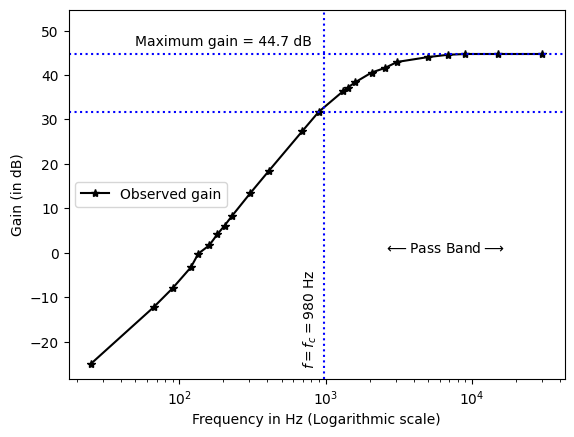
\includegraphics[width=1\columnwidth]{images/high_pass_output.png}
        \caption{Bode plot (Gain vs frequency) for Table \ref{tab:2}}
        \label{highoutput}
    \end{figure}

From the graph, the observed value of the cutoff frequency is around 980 Hz. There is some deviation in the expected value from the experimental value, which could be due to various reasons as mentioned previously. 
